\section{Uygulama II}
Bu bölümde SAP2000 OAPI kullanılarak 4 açıklıklı, 8 katlı basit bir çelik çerçevenin kesit optimizasyonu gerçekleştirilecektir. Optimizasyon işlemi için tavlama benzetimi algoritması kullanılacak ve LRFD yöntemine göre tasarım yapılacaktır.

\sidenote{
    
\qrcode[height=1in]{https://github.com/btayfur/structural-optimization/blob/main/Code/Examples/Exmp7/}}

\subsection{Çelik çerçeve modeli}
Model, 4 açıklıklı (5m açıklık mesafesi) ve 8 katlı (3m kat yüksekliği) bir çelik çerçeve yapıdan oluşmaktadır. Her katta açıklık üzerinde 40 kN/m düzgün yayılı yük bulunmaktadır. Tüm mesnetler ankastre olarak modellenmiştir. Yapıda Grade 36 çeliği kullanılmaktadır. Kirişlerin serbest burkulma boyu, kiriş uzunluğunun 1/5'i olarak kabul edilmiştir. SAP2000 Steel Design aracı kullanılarak tasarım ve optimizasyon işlemleri gerçekleştirilecektir.

\begin{figure}[H]
    \centering
    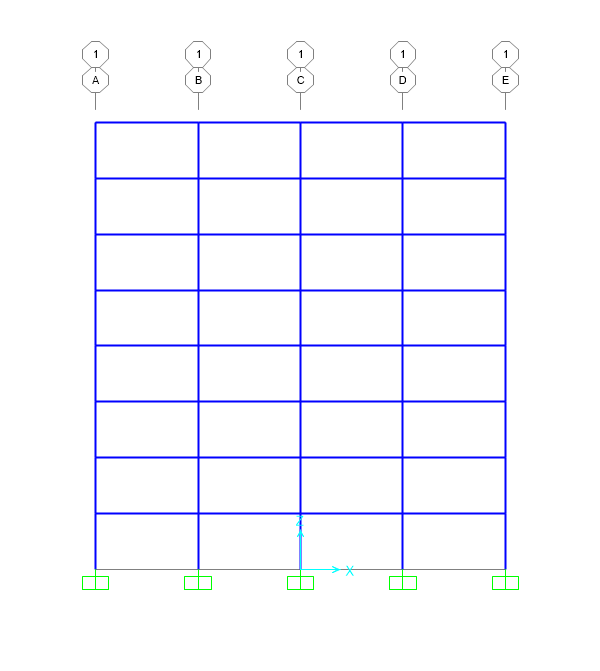
\includegraphics[width=0.8\textwidth]{weeks_new/imgs/exmp7_fig2.png}
    \caption{Çelik çerçeve modeli}
    \label{fig:model}
\end{figure}

\begin{figure}[H]
    \centering
    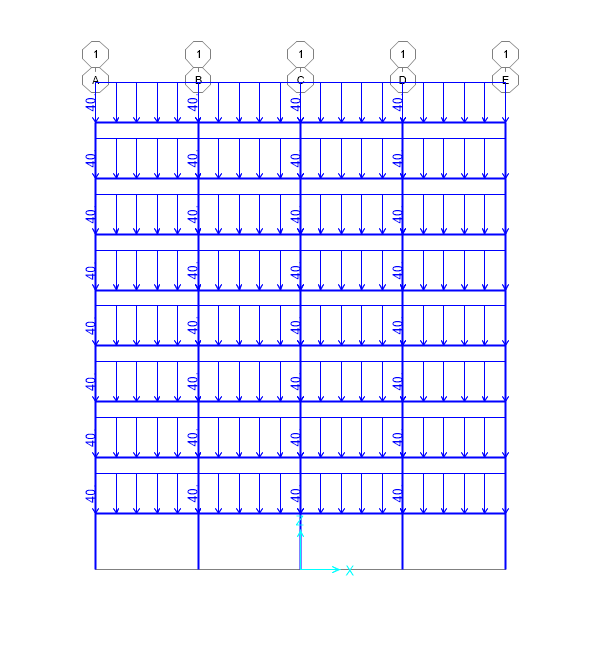
\includegraphics[width=0.8\textwidth]{weeks_new/imgs/exmp7_fig1.png}
    \caption{Yükleme Durumu}
    \label{fig:loading}
\end{figure}

\begin{figure}[H]
    \centering
    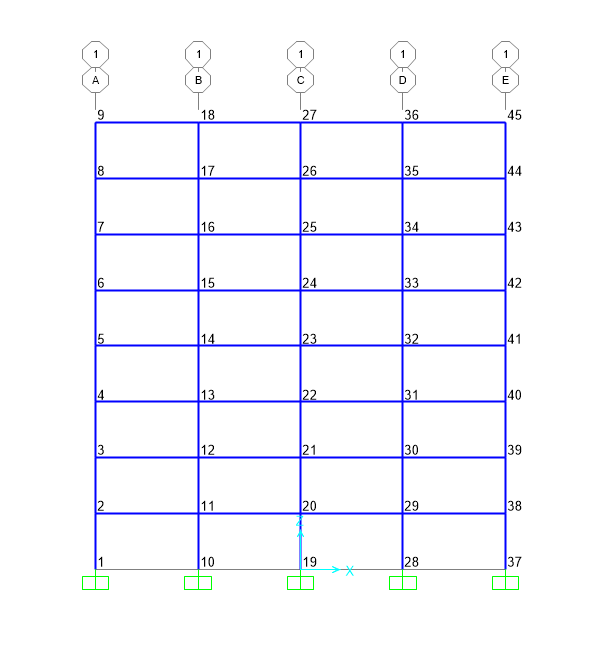
\includegraphics[width=0.8\textwidth]{weeks_new/imgs/exmp7_fig3.png}
    \caption{Düğüm noktalarının numaralandırılması}
    \label{fig:joints}
\end{figure}

\subsection{Kesit gruplandırması}
Yapıda kolon ve kirişler iki katta bir değişecek şekilde gruplandırılmıştır. Bu durumda toplam 4 kolon grubu ve 4 kiriş grubu bulunmaktadır. Her grup için farklı kesit seçimleri yapılacak ve optimizasyon sürecinde bu grupların kesitleri optimize edilecektir.

\subsubsection{Seçilebilir parametrelerin belirlenmesi}
Optimizasyon sürecinde kullanılacak kesit listesi, AISC kataloğundan seçilen W profillerinden oluşmaktadır. Kesit listesi W12'den W33'ye kadar farklı boyutlardaki profilleri içermektedir. Her grup için bu listeden uygun kesit seçimi yapılacak ve optimizasyon algoritması tarafından en uygun kesitler belirlenecektir.

\subsection{Optimizasyon}

\subsubsection{Amaç Fonksiyonu}
Optimizasyon sürecinde amaç fonksiyonu, yapının toplam ağırlığını minimize etmek olarak belirlenmiştir. Bu sayede hem ekonomik bir çözüm elde edilecek hem de yapının performansı optimize edilecektir.
Yapı ağırlığının hesaplamak için model içinde "weight" adlı bir "load case" oluşturulmuştur. Bu "load case" başka bir kuvvet barındırmadığından z eksenindeki mesnet reaksiyonları toplamı yapı ağırlığını verir. Bununla birlikte birçok yapısal optimizasyon probleminde olduğu gibi bu problemde de amaç fonksiyonu aşağıdaki gibi ifade edilebilir:

\begin{equation}
    f(x) = \sum_{i=1}^{n} \rho_i \cdot A_i \cdot L_i
\end{equation}
Burada $\rho_i$ kesit ağırlığını, $A_i$ kesit alanını ve $L_i$ kesit uzunluğunu ifade etmektedir. \sidenote{
    W kesitlerin kullanıldığı daha karmaşık problemlerde kesit isimlendirmesinden faydalanılabilir. Örneğin W12$\times$35 kesitinin $x35$ kısmı birim uzunluk başına ağırlığı ifade eder. Ancak bu değerlerin SI birimlerine çevrilmesi gerekmektedir.
}


\subsubsection{Sınırlayıcılar}
Optimizasyon sürecinde aşağıdaki sınırlayıcılar SAP2000 Çeelik Tasarım aracı kullanılarak gerçekleştirilir. VerifyPassed() metodu, yönetmelik şartlarını sağlamayan çerçeve elemanı sayısını döndürür. Arka planda ise burkulma boyundan genel bileşik denklemlere kadar tüm kontroller gerçekleştirilir. Ancak birçok optimizasyon çalışmasında -özellikle hız amacıyla OAPI ve benzeri araçların kullanılmadığı- aşağıdaki bileşik etki denklemleri kullanılarak kontroller sağlanır:
\begin{equation}
    \frac{P_u}{\phi_c P_n} \geq 0.2; \quad c_1=\frac{P_u}{\phi_c P_n} + \frac{8}{9} \left(\frac{M_{ux}}{\phi_b M_{nx}} + \frac{M_{uy}}{\phi_b M_{ny}}\right) 
\end{equation}
\begin{equation}
    \frac{P_u}{\phi_c P_n} < 0.2; \quad c_2=\frac{P_u}{\phi_c P_n} +  \left(\frac{M_{ux}}{\phi_b M_{nx}} + \frac{M_{uy}}{\phi_b M_{ny}}\right) 
\end{equation}
\begin{equation}
    \forall i: c_i \leq 1.0
\end{equation}

\subsection{Optimizasyon Sonuçları}
Tavlama benzetimi algoritması daha önce bahsedildiği gibi bir stokastik yöntemdir. Bu nedenle her çalıştırmada farklı sonuçların elde edilmesi doğaldır. Fakat araştırma amacıyla yapılan bir çalışmada algoritmanın tutarlığını sağlamak için genellikle çok sayıda çalıştırma yapılarak algoritmanın genel başarımı daha iyi anlaşılabilir. Bu örnekte yalnızca bir kez ve düşük sayılı iterasyon sınırı ile çalıştırma yapılacak ve sonuçları incelenecektir. Ancak yeterli analiz süresi tanındığında, örnek kapsamındaki kod da kolayca bu bağlamda değiştirilebilir.

\begin{figure}[H]
    \centering
    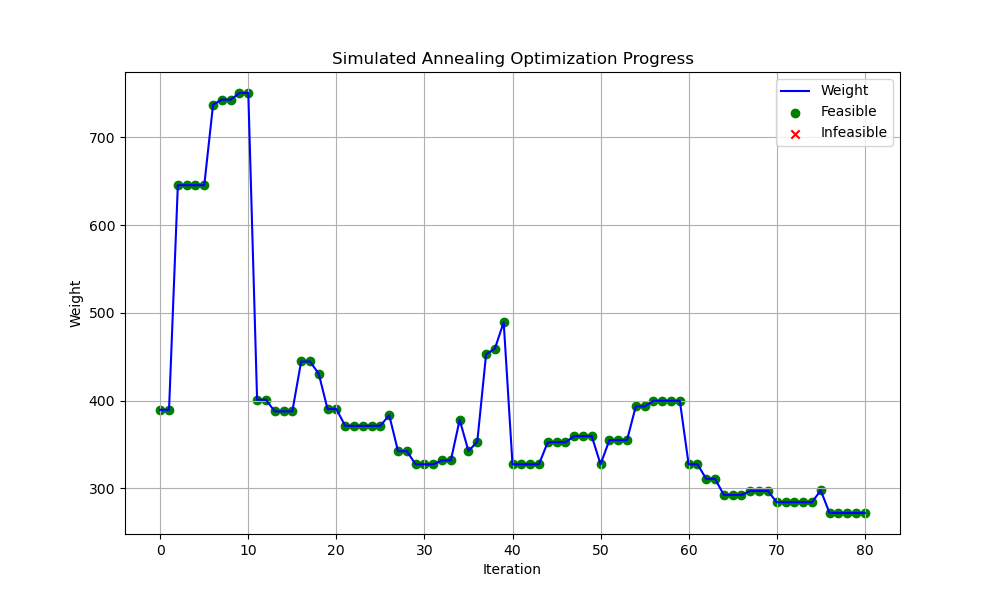
\includegraphics[width=0.8\textwidth]{weeks_new/imgs/exmp7_fig4.png}
    \caption{Yapı ağırlığının optimizasyon süresince değişimi}
    \label{fig:weight_change}
\end{figure}

\begin{table}
    \caption{Kiriş ve kolon kesitleri}
\end{table}

\begin{figure}[H]
    \centering
    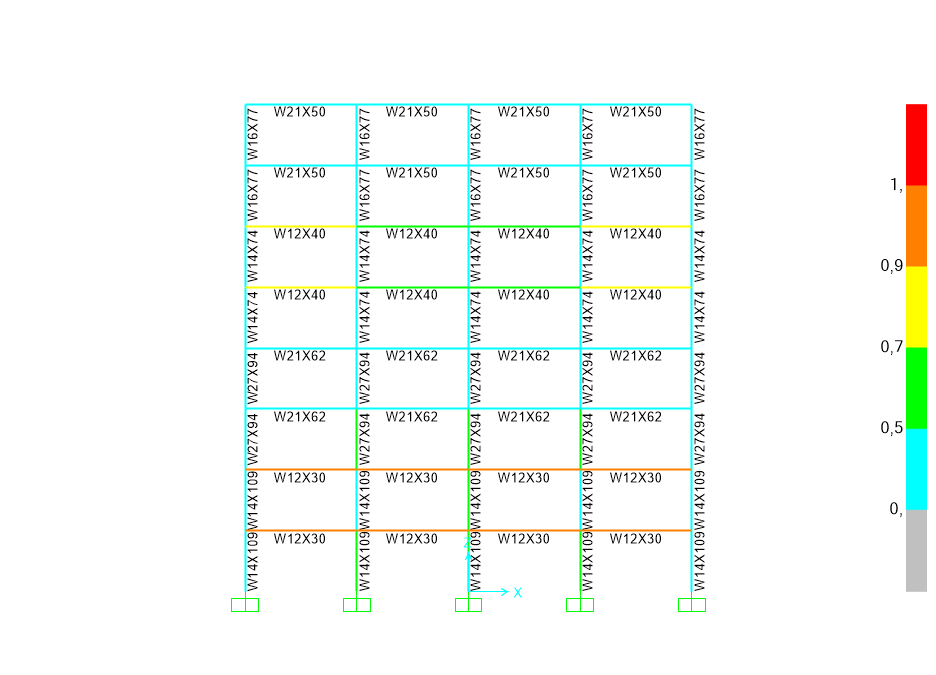
\includegraphics[width=0.8\textwidth]{weeks_new/imgs/exmp7_fig5.png}
    \caption{Optimum tasarımın Talep/Kapasite Oranı gösterimi}
    \label{fig:dcr_values}
\end{figure}





